\chapter{Kehidupan Sepanjang Musim}\label{ch:g6:life-through-seasons}

Fotolah pohon berangan yang sama pada tanggal satu setiap bulan lalu
sematkan kedua belas gambarnya berderet: dahan telanjang, \omterm{def:g6:life-through-seasons:buds}{kuncup},
\omterm{def:g1:plants-around-us:parts}{daun}, ``lilin'' \omterm{def:g3:flowers-fruits-seeds:parts}{bunga}, \omterm{prop:g3:flowers-fruits-seeds:transform}{buah} berangan, warna emas, lalu dahan telanjang
lagi. Tidak ada yang berpindah --- pohonnya berdiri diam sepanjang
tahun --- namun segalanya berubah. \Cref{ch:g3:animals-through-seasons}
mengikuti \omterm{def:g1:animals-around-us:animal}{hewannya} sepanjang tahun; sekarang, dengan \omterm{def:g1:the-five-senses:sense}{mata} seorang
penyurvei, kita mengikuti seluruh \omterm{def:g6:exploring-our-environment:components}{lingkungannya}, \omterm{def:g1:plants-around-us:plant}{tumbuhan} lebih
dahulu.

\section{Lingkungan berubah bersama musimnya}

\begin{proposition}[Perubahan musiman kondisinya]\label{prop:g6:life-through-seasons:conditions}
Sepanjang tahun, \omterm{def:g6:exploring-our-environment:conditions}{kondisi} sebuah \omterm{def:g6:exploring-our-environment:components}{lingkungan}
(\cref{def:g6:exploring-our-environment:conditions}) berayun lebar:
harinya memendek lalu memanjang, \omterm{def:g6:exploring-our-environment:conditions}{suhunya} turun lalu naik, \omterm{def:g6:exploring-our-environment:conditions}{kelembapan}
tanahnya mengikuti hujan dan kemarau. Sebuah lokasi yang disurvei pada
bulan Januari dan pada bulan Juni memberi dua baris yang berbeda dalam
tabelnya --- sehingga, menurut
\cref{prop:g6:exploring-our-environment:decide}, harapkanlah dua
rombongan penghuni yang berbeda.
\end{proposition}
\admitted

\begin{example}[Satu pagar tanaman, dua survei]\label{ex:g6:life-through-seasons:hedge}
Pagar tanaman di jalan kecil itu, yang disurvei dua kali. Juni: \omterm{def:g1:plants-around-us:parts}{daunnya}
lebat, sepuluh \omterm{def:g5:biodiversity:species}{spesies} \omterm{def:g1:plants-around-us:plant}{tumbuhan} berbunga di kakinya, lebah berdengung
keras, \omterm{prop:g3:sorting-living-things:groups}{burung} hitam bersarang, siput muncul sesudah hujan. Januari:
\omterm{def:g1:plants-around-us:tree}{ranting} telanjang, warna hijau menyusut tinggal ivi dan \omterm{prop:g4:plants-without-seeds:damp}{lumut}, tidak
ada \omterm{prop:g3:sorting-living-things:groups}{serangga} yang terbang, \omterm{prop:g3:sorting-living-things:groups}{burung} hitam mencari makan di dalam
serasah, siput tersegel di dalam \omterm{def:g1:animals-around-us:covering}{cangkangnya} jauh di dalam tebing
tanahnya. Tempat yang sama, daftar komponen yang sama --- hidup,
mineral, jejak --- tetapi lajur yang hidup sudah berubah rupa.
\end{example}

\section{Bagaimana tumbuhan melewati musim yang buruk}

\begin{definition}[Meranggas dan selalu hijau]\label{def:g6:life-through-seasons:trees}
Pohon terbagi menurut jawaban musim dinginnya:
\begin{itemize}
  \item pohon \emph{meranggas}\index{meranggas} --- pohon ek, berangan,
        beech --- menanggalkan seluruh \omterm{def:g1:plants-around-us:parts}{daunnya} pada musim gugur lalu
        berdiri telanjang;
  \item pohon \emph{selalu hijau}\index{selalu hijau} --- pinus, holi,
        ivi di tembok --- mempertahankan \omterm{def:g1:plants-around-us:parts}{daun} yang bekerja sepanjang
        musim dingin, biasanya \omterm{def:g1:plants-around-us:parts}{daun} yang liat, berlilin atau berbentuk
        jarum (\cref{prop:g3:sorting-living-things:plants} sudah
        berjumpa dengan jarumnya).
\end{itemize}
\end{definition}

\begin{definition}[Kuncup]\label{def:g6:life-through-seasons:buds}
Pohon \omterm{def:g6:life-through-seasons:trees}{meranggas} pada musim dingin tidaklah mati: musim semi berikutnya
sudah terkemas di \omterm{def:g1:plants-around-us:tree}{rantingnya} sebagai \emph{kuncup}\index{kuncup} ---
tunas lengkap yang mungil, \omterm{def:g1:plants-around-us:parts}{daunnya} terlipat kecil, terbungkus \omterm{def:g1:animals-around-us:covering}{sisik}
yang tahan cuaca. \omterm{def:g1:plants-around-us:parts}{Daun} ``baru'' musim semi dibangun pada musim panas
sebelumnya; kuncupnya adalah gudang musim dingin baginya.
\end{definition}

\begin{example}[Membuka kuncup berangan kuda]\label{ex:g6:life-through-seasons:bud}
\omterm{def:g6:life-through-seasons:buds}{Kuncup} besar dan lengket milik berangan kuda terbuka dengan baik di
bawah sebilah pisau (pekerjaan untuk orang dewasa): di bawah \omterm{def:g1:animals-around-us:covering}{sisiknya}
yang berpernis, terkemas dalam \omterm{def:g1:animals-around-us:covering}{bulu} halus mirip kapas, terbaring \omterm{def:g1:plants-around-us:parts}{daun}
terlipat yang mungil --- sempurna, pucat, menunggu. Sebuah \omterm{def:g1:plants-around-us:tree}{ranting}
yang dipotong pada bulan Februari lalu ditegakkan dalam air di dalam
ruangan ``berdaun'' berminggu-minggu lebih awal: tunasnya sudah
selesai; hanya kehangatannya yang hilang.
\end{example}

\begin{omfigure}
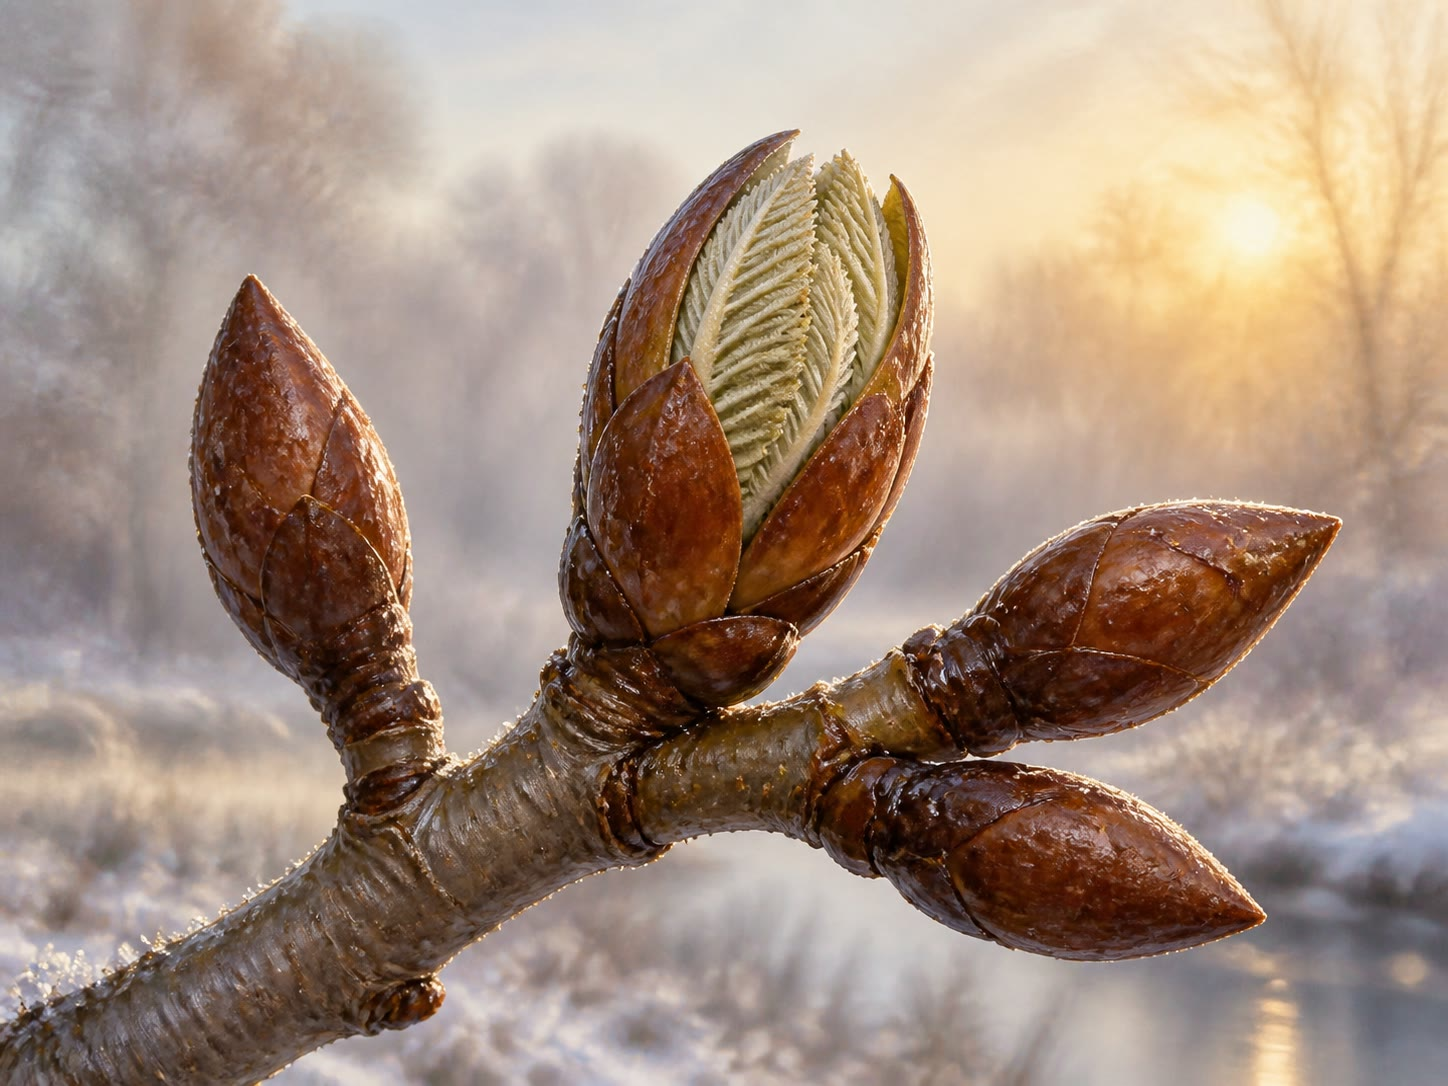
\includegraphics[width=0.56\linewidth]{images/book1/ai/g6-seasons-buds.jpg}

{\small Gudang musim dingin, yang terbuka: di dalam \omterm{def:g1:animals-around-us:covering}{sisik} \omterm{def:g6:life-through-seasons:buds}{kuncup}
berpernis milik berangan kuda, \omterm{def:g1:plants-around-us:parts}{daun} musim semi berikutnya terbaring
terlipat dan sudah selesai.}
\end{omfigure}

\begin{proposition}[Jawaban musim dingin lapisan tumbuhan kecil]\label{prop:g6:life-through-seasons:herbs}
\omterm{def:g1:plants-around-us:plant}{Tumbuhan} yang lebih kecil punya siasatnya sendiri:
\begin{itemize}
  \item \emph{tumbuhan semusim}\index{tumbuhan semusim} --- \omterm{def:g3:flowers-fruits-seeds:parts}{bunga} popi,
        kacang --- mati seluruhnya pada musim gugur lalu melewati musim
        dingin sebagai \emph{\omterm{def:g2:from-seed-to-plant:seed}{biji}} (\cref{prop:g2:from-seed-to-plant:needs}:
        sebutir \omterm{def:g2:from-seed-to-plant:seed}{biji} menunggui dinginnya dengan aman);
  \item \emph{tumbuhan tahunan}\index{tumbuhan tahunan} --- \omterm{def:g3:flowers-fruits-seeds:parts}{bunga}
        narsis, jombang --- membiarkan bagian atasnya mati lalu
        menunggu di bawah tanah sebagai \omterm{ex:g4:plants-without-seeds:bulbtuber}{umbi lapis}, \omterm{ex:g4:plants-without-seeds:bulbtuber}{umbi batang} atau
        pangkal \omterm{def:g1:plants-around-us:parts}{akar} yang liat (gudang pada
        \cref{ex:g4:plants-without-seeds:bulbtuber}, yang sedang
        bertugas musim dingin);
  \item yang \omterm{def:g6:life-through-seasons:trees}{selalu hijau} di permukaan tanah --- \omterm{prop:g4:plants-without-seeds:damp}{lumut}, ivi --- sekadar
        bertahan.
\end{itemize}
\end{proposition}
\admitted

\begin{example}[Ke mana perginya bunga narsisnya?]\label{ex:g6:life-through-seasons:daffodil}
Petak \omterm{def:g3:flowers-fruits-seeds:parts}{bunga} narsisnya berbunga pada bulan Maret, menguning pada bulan
Mei, dan menjelang Juli lenyap tanpa jejak --- namun pada bulan Maret
berikutnya ia kembali, lebih rapat. Sepanjang musim panas, musim gugur
dan musim dingin ia ada sebagai \omterm{ex:g4:plants-without-seeds:bulbtuber}{umbi lapis} di bawah halaman rumputnya:
\omterm{def:g1:plants-around-us:plant}{tumbuhannya} tidak pernah pergi; ia menarik diri ke gudangnya.
\end{example}

\section{Penanggalan hewan, ditinjau ulang}

\begin{proposition}[Jawaban hewan, dalam istilah survei]\label{prop:g6:life-through-seasons:animals}
Ketiga siasat pada \cref{ch:g3:animals-through-seasons} ---
\omterm{def:g3:animals-through-seasons:migration}{bermigrasi}, \omterm{def:g3:animals-through-seasons:hibernation}{berhibernasi}, \omterm{def:g3:animals-through-seasons:active}{tetap aktif} --- sekarang terbaca sebagai
jawaban atas perubahan yang disurvei: tiap \omterm{def:g5:biodiversity:species}{spesies} mengikuti \omterm{def:g6:exploring-our-environment:conditions}{kondisi}
dan makanan yang dibutuhkannya sendiri.
\begin{itemize}
  \item \omterm{prop:g3:sorting-living-things:groups}{burung} layang-layang mengikuti persediaan makanannya ke tempat
        \omterm{def:g6:exploring-our-environment:conditions}{kondisinya} menjaga \omterm{prop:g3:sorting-living-things:groups}{serangga} tetap terbang;
  \item landak dan siput yang tersegel menunggui bulan-bulan yang
        tidak dapat dilalui tubuhnya dengan bekerja;
  \item \omterm{prop:g3:sorting-living-things:groups}{serangga} menambahkan jawaban keempat: kebanyakan melewati
        musim dingin sebagai \emph{\omterm{def:g2:animals-grow-up:born}{telur}, larva atau \omterm{ex:g2:animals-grow-up:butterfly}{kepompong}}
        (\cref{ex:g2:animals-grow-up:butterfly}) yang terselip di
        tanah, kulit kayu atau serasah --- yang dewasa mati, dan
        \omterm{def:g5:biodiversity:species}{spesiesnya} melewati musim dingin sebagai tahap mudanya.
\end{itemize}
\end{proposition}
\admitted

\begin{example}[Di mana serangga bulan Juni pada bulan Januari]\label{ex:g6:life-through-seasons:insects}
Pagar tanaman bulan Januari tidak memperlihatkan seekor \omterm{prop:g3:sorting-living-things:groups}{serangga} pun
--- namun \omterm{prop:g3:sorting-living-things:groups}{serangga} bulan Juni semuanya hadir: kupu-kupunya sebagai
\omterm{ex:g2:animals-grow-up:butterfly}{kepompong} di bawah batu puncak temboknya, belalangnya sebagai \omterm{def:g2:animals-grow-up:born}{telur} di
dalam tanah, kepiknya sebagai kumpulan dewasa yang \omterm{prop:g1:healthy-habits:needs}{tidur} berimpitan
jauh di dalam serasah, lebahnya sebagai gerombolan rapat yang hangat
di dalam sarang. Survei bulan Juni berjalan-jalan; survei bulan
Januari harus menggali, mengangkat dan mengintip --- penghuninya
berubah \emph{wujud}, bukan alamat.
\end{example}

\begin{method}[Mensurvei sepanjang tahun]\label{met:g6:life-through-seasons:yearsurvey}
Untuk mempelajari kehidupan musiman sebuah lokasi:
\begin{enumerate}
  \item surveilah lokasi bertanda yang sama
        (\cref{met:g6:exploring-our-environment:survey})
        satu kali tiap musim --- petak yang sama, alat yang sama,
        waktu pencarian yang sama;
  \item catatlah \omterm{def:g6:exploring-our-environment:conditions}{kondisinya} \emph{dan} penghuninya setiap kali;
        fotolah lokasinya dari tempat yang sama;
  \item carilah wujud tersembunyi musim dingin dengan sengaja:
        \omterm{def:g6:life-through-seasons:buds}{kuncup}, \omterm{ex:g4:plants-without-seeds:bulbtuber}{umbi lapis}, \omterm{def:g2:animals-grow-up:born}{telur}, \omterm{ex:g2:animals-grow-up:butterfly}{kepompong}, siput yang tersegel ---
        dan kembalikanlah setiap penutupnya;
  \item bentangkan keempat surveinya berdampingan: pasangkan tiap
        perubahan penghuninya dengan sebuah perubahan \omterm{def:g6:exploring-our-environment:conditions}{kondisinya}, lalu
        sebutkan wujud musim dingin atau tujuan tiap yang absen.
\end{enumerate}
\end{method}

\begin{remark}[Tidak ada yang sekadar lenyap]\label{rem:g6:life-through-seasons:vanish}
Tabel sepanjang tahun itu mengajarkan satu aturan yang dalam: tidak
ada \omterm{def:g5:biodiversity:species}{spesies} pada survei bulan Juni yang sekadar berhenti ada. Tiap
\omterm{def:g5:biodiversity:species}{spesiesnya} berada di tempat lain (\omterm{def:g3:animals-through-seasons:migration}{bermigrasi}), tertidur
(\omterm{def:g3:animals-through-seasons:hibernation}{berhibernasi}), di dalam gudang (\omterm{ex:g4:plants-without-seeds:bulbtuber}{umbi lapis}, \omterm{def:g2:from-seed-to-plant:seed}{biji}), atau dalam tahap
kehidupan yang lain (\omterm{def:g2:animals-grow-up:born}{telur}, \omterm{ex:g2:animals-grow-up:butterfly}{kepompong}). ``Hilang'' tidak pernah
menjadi jawaban yang lengkap dalam \omterm{def:g1:living-or-not:living}{biologi} --- pertanyaan lanjutannya
selalu \emph{hilang ke mana, sebagai apa?}
\end{remark}

\section{Latihan}

\begin{exercise}[$\star$]\label{exo:g6:life-through-seasons:1}
\omterm{def:g6:exploring-our-environment:conditions}{Kondisi} lokasi mana yang berayun bersama musimnya? Sebutkan tiga.
\end{exercise}

\begin{exercise}[$\star$]\label{exo:g6:life-through-seasons:2}
\omterm{def:g6:life-through-seasons:trees}{Meranggas} atau \omterm{def:g6:life-through-seasons:trees}{selalu hijau}: pohon ek, pinus, beech, holi, berangan
kuda? Apa arti tiap katanya?
\end{exercise}

\begin{exercise}[$\star$]\label{exo:g6:life-through-seasons:3}
Apa yang ada di dalam sebuah \omterm{def:g6:life-through-seasons:buds}{kuncup} musim dingin, dan kapan ia
dibangun?
\end{exercise}

\begin{exercise}[$\star$]\label{exo:g6:life-through-seasons:4}
Bagaimana \omterm{prop:g6:life-through-seasons:herbs}{tumbuhan semusim} melewati musim dingin? Dan \omterm{prop:g6:life-through-seasons:herbs}{tumbuhan tahunan}
seperti \omterm{def:g3:flowers-fruits-seeds:parts}{bunga} narsis?
\end{exercise}

\begin{exercise}[$\star$]\label{exo:g6:life-through-seasons:5}
Jelaskan \omterm{def:g1:plants-around-us:tree}{ranting} bulan Februari pada \cref{ex:g6:life-through-seasons:bud}:
mengapa ia dapat berdaun berminggu-minggu lebih awal di dalam ruangan?
\end{exercise}

\begin{exercise}[$\star$]\label{exo:g6:life-through-seasons:6}
Berikan keempat jawaban musim dingin \omterm{def:g1:animals-around-us:animal}{hewan}, masing-masing dengan satu
\omterm{def:g5:biodiversity:species}{spesies}.
\end{exercise}

\begin{exercise}[$\star\star$]\label{exo:g6:life-through-seasons:7}
Untuk tiap penghuni pagar tanaman bulan Juni, sebutkan wujud dan
alamat bulan Januarinya: kupu-kupu, belalang, kepik, siput, \omterm{prop:g3:sorting-living-things:groups}{burung}
layang-layang.
\end{exercise}

\begin{exercise}[$\star\star$]\label{exo:g6:life-through-seasons:8}
Mengapa keempat survei musimannya harus memakai lokasi, alat dan waktu
pencarian yang sama? Aturan \cref{ch:g6:exploring-our-environment}
yang mana yang sedang bekerja?
\end{exercise}

\begin{exercise}[$\star\star$]\label{exo:g6:life-through-seasons:9}
Survei pagar tanaman bulan Januari mendaftarkan \omterm{def:g6:exploring-our-environment:components}{makhluk hidup} jauh
lebih sedikit daripada bulan Juni. Berikan dua alasan mengapa
perbedaannya melebih-lebihkan kehilangan yang sesungguhnya, dengan
memakai \cref{ex:g6:life-through-seasons:insects}.
\end{exercise}

\begin{exercise}[$\star\star$]\label{exo:g6:life-through-seasons:10}
Seorang tukang kebun menggali tanah \omterm{def:g3:flowers-fruits-seeds:parts}{bunga} narsis yang ``mati'' pada
bulan Agustus lalu menemukan \omterm{ex:g4:plants-without-seeds:bulbtuber}{umbi lapis} yang keras. Terjemahkan
temuannya dengan \cref{prop:g6:life-through-seasons:herbs}: dalam
keadaan apa \omterm{def:g1:plants-around-us:plant}{tumbuhannya}, dan apa yang akan dilakukan umbinya pada
bulan Maret?
\end{exercise}

\begin{exercise}[$\star\star$]\label{exo:g6:life-through-seasons:11}
Terapkan \cref{rem:g6:life-through-seasons:vanish}: katak sebuah kolam
tidak dapat ditemukan di mana pun pada bulan Januari. Berikan kedua
pertanyaan yang harus diajukan, dan jawaban kodok-dan-kataknya.
\end{exercise}

\begin{exercise}[$\star\star\star$]\label{exo:g6:life-through-seasons:12}
\omterm{def:g1:plants-around-us:parts}{Daun} yang \omterm{def:g6:life-through-seasons:trees}{selalu hijau} itu liat, berlilin atau berbentuk jarum; \omterm{def:g1:plants-around-us:parts}{daun}
yang \omterm{def:g6:life-through-seasons:trees}{meranggas} lebar dan tipis. Ajukanlah masalah musim dingin apa
yang dijawab oleh bangunan \omterm{def:g1:plants-around-us:parts}{daun} yang \omterm{def:g6:life-through-seasons:trees}{selalu hijau} itu (pikirkan
masalah air kutu kayu secara terbalik), dan mengapa pohon yang
\omterm{def:g6:life-through-seasons:trees}{meranggas} lebih memilih menanggalkan \omterm{def:g1:plants-around-us:parts}{daunnya} yang tipis.
\end{exercise}

\section{Soal: Dua Belas Foto}

\begin{problem}[{Soal akhir pekan --- setahun perjalanan pohon
berangan, yang dibaca bingkai demi bingkai}]\label{pb:g6:life-through-seasons:1}
Lena memotret pohon berangan di dekat gerbang pada tanggal satu setiap
bulan selama setahun, lalu menyematkan kedua belas cetakannya
berderet. Di bawah tiap cetakan ia mencatat panjang harinya dan \omterm{def:g6:exploring-our-environment:conditions}{suhu}
paginya.

\medskip\noindent\textbf{Bagian I --- Membaca deretnya.}
\begin{enumerate}
  \item Bulan Januari dan Desember memperlihatkan dahan yang telanjang.
        Apa, di \omterm{def:g1:plants-around-us:tree}{rantingnya}, yang membuktikan bahwa pohonnya hidup dan
        siap menyongsong musim semi pada kedua bingkai itu?
  \item Di antara dua bingkai mana \omterm{def:g6:life-through-seasons:buds}{kuncupnya} merekah? Catatan Lena di
        situ berbunyi: harinya
        $11$--$13$ jam, paginya
        $8$--\qty{12}{\degreeCelsius}. \omterm{def:g6:exploring-our-environment:conditions}{Kondisi} yang berubah mana yang
        sedang dijawab pohonnya?
  \item Bingkai bulan Mei memperlihatkan ``lilin'' \omterm{def:g3:flowers-fruits-seeds:parts}{bunga} putih yang
        tegak. Dengan memakai \cref{ch:g3:flowers-fruits-seeds} (atau
        \cref{ch:g5:flower-to-fruit}), apa yang harus berkunjung di
        antara bingkai bulan Mei dan bulan September agar \omterm{prop:g3:flowers-fruits-seeds:transform}{buah} berangan
        bulan Oktober ada --- dan \omterm{prop:g3:flowers-fruits-seeds:transform}{buah} berangan itu apa, tepatnya?
  \item Bingkai bulan Oktober memperlihatkan \omterm{def:g1:plants-around-us:parts}{daun} keemasan; bingkai
        bulan November, dahan telanjang dan hamparan cokelat di
        bawahnya. Sebutkan jenis pohonnya menurut
        \cref{def:g6:life-through-seasons:trees}, dan di mana musim
        semi berikutnya disimpan sepanjang bingkai yang menyusul.
\end{enumerate}

\medskip\noindent\textbf{Bagian II --- Tetangga pohonnya.}
\begin{enumerate}[resume]
  \item Di bawah pohonnya, bingkai bulan Maret menangkap sepetak \omterm{def:g3:flowers-fruits-seeds:parts}{bunga}
        narsis yang tidak ada pada bingkai bulan Juli. Di mana
        petaknya pada bulan Juli, dan dalam wujud apa?
  \item \omterm{def:g3:flowers-fruits-seeds:parts}{Bunga} popi berjajar di tepi jalan setapak pada bulan Juni; pada
        bingkai bulan Januari tempatnya berupa tanah kosong. Dalam
        wujud apa \omterm{def:g3:flowers-fruits-seeds:parts}{bunga} popinya hadir pada bulan Januari, dan dengan
        siasat yang mana pada
        \cref{prop:g6:life-through-seasons:herbs}?
  \item Bingkai bulan Juni menangkap seekor \omterm{prop:g3:sorting-living-things:groups}{burung} layang-layang di
        atas pohonnya dan lebah pada \omterm{def:g3:flowers-fruits-seeds:parts}{bunga} di bawahnya; keduanya tidak
        muncul dari bulan November sampai Februari. Untuk
        masing-masing, sebutkan di mana ia berada waktu itu, dan
        sebagai apa.
  \item Seekor \omterm{prop:g3:sorting-living-things:groups}{burung} murai muncul pada setiap bingkainya. Siasat \omterm{def:g1:animals-around-us:animal}{hewan}
        yang mana itu, dan apa yang harus dikelola \omterm{prop:g3:sorting-living-things:groups}{burung} murainya sepanjang
        musim dingin, yang dihindari \omterm{prop:g3:sorting-living-things:groups}{burung} layang-layang dengan pergi?
\end{enumerate}

\medskip\noindent\textbf{Bagian III --- Aturan deretnya.}
\begin{enumerate}[resume]
  \item Lena merangkum: ``tahun pohonnya mengikuti tahun \omterm{def:g6:exploring-our-environment:conditions}{kondisinya}.''
        Dukunglah ia dengan dua pemasangan antara sebuah perubahan
        pohonnya dari bingkai ke bingkai dan sebuah perubahan pada
        catatan panjang hari serta \omterm{def:g6:exploring-our-environment:conditions}{suhunya}.
  \item Adik lelakinya berkata bahwa petak \omterm{def:g3:flowers-fruits-seeds:parts}{bunga} narsis bulan Juli
        ``mati''. Betulkan ia dengan
        \cref{rem:g6:life-through-seasons:vanish} --- lalu nyatakan
        pertanyaan lanjutan yang selalu pantas diterima kata
        ``hilang'' miliknya.
  \item Ramalkan bingkai ke-13 --- foto bulan Januari tahun berikutnya
        --- dengan terperinci: dahan, \omterm{def:g1:plants-around-us:tree}{ranting}, tanah di bawahnya.
        Bagian ramalanmu yang mana yang cukup pasti untuk
        dipertaruhkan, dan mengapa?
  \item Sebuah \omterm{def:g1:plants-around-us:tree}{ranting} berangan, yang dipotong pada bulan Februari lalu
        ditegakkan dalam air hangat di dalam ruangan, berdaun dalam
        tiga minggu. Apa yang ditunjukkannya tentang \omterm{def:g6:exploring-our-environment:conditions}{kondisi}
        \emph{yang mana} yang ditunggu \omterm{def:g6:life-through-seasons:buds}{kuncupnya} --- lalu rancanglah
        uji adil dua \omterm{def:g1:plants-around-us:tree}{ranting}
        (\cref{met:g4:what-plants-need:fairtest}) yang akan
        memastikannya.
\end{enumerate}
\end{problem}
